\subsection{Class Diagram}
\begin{center}
	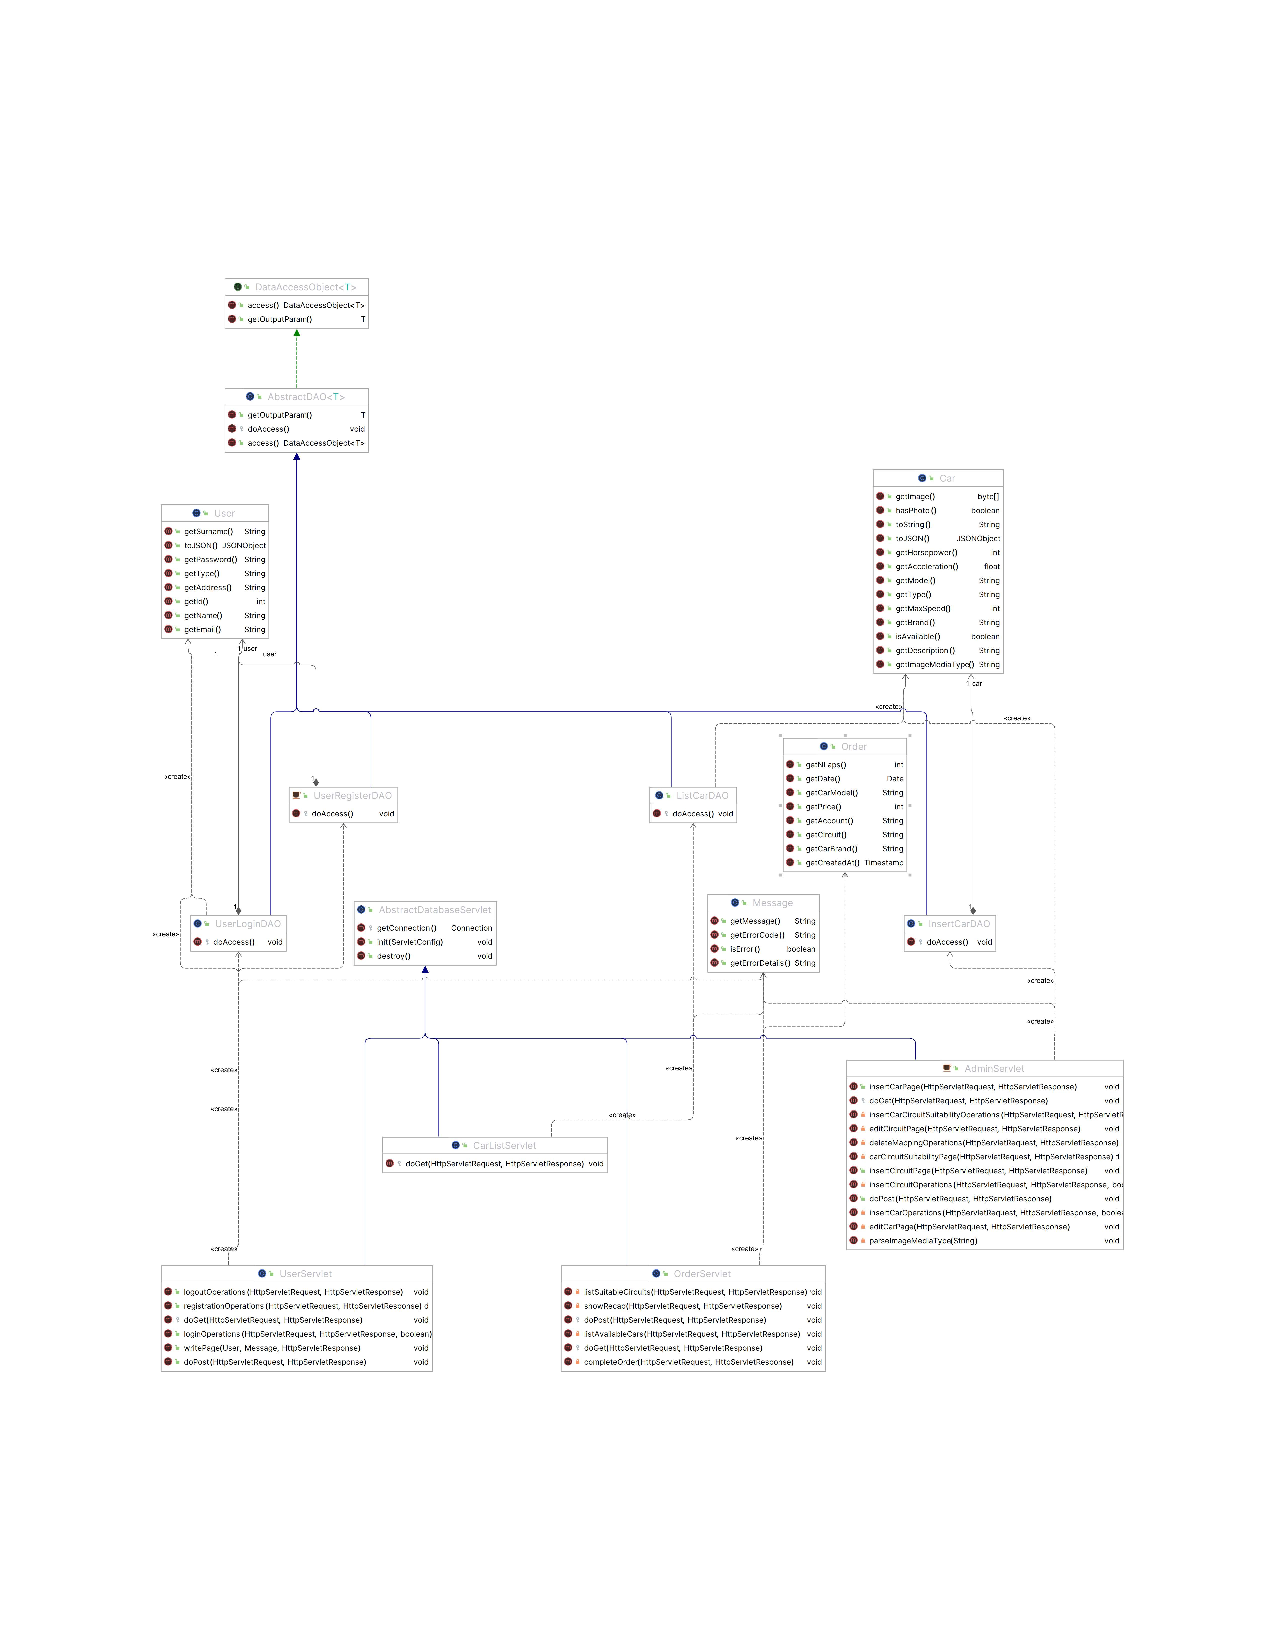
\includegraphics[scale=0.65]{ClassDiagram.pdf}
	\captionof{figure}{Class diagram of WACAR}
	\label{ERSchema}
\end{center}

The class diagram includes some of the classes utilized in WaCar. Each servlet extends the \texttt{AbstractDatabaseServlet}, necessary for acquiring the database connection. Four servlets are delineated:

\textbf{UserServlet}: Handles user operations such as login, registration, and logout. It implements the \texttt{doGet} and \texttt{doPost} methods to manage HTTP requests. Not all URIs are freely accessible: while login and registration are, accessing user information requires authentication; otherwise, users are redirected to the login page using the corresponding filter (this is also valid for OrderServlet and AdminServlet).

\begin{itemize}
    \item \texttt{doGet}: Manages GET requests related to user authentication. Supported operations include login, registration, and logout. Authenticated users are redirected to the user page; otherwise, appropriate error messages are returned. For example, when the URI ends with "login/", the current session is invalidated and the request is forwarded to the login page.
    \item \texttt{doPost}: Manages POST requests related to user authentication. Supports login and registration operations, handling client-sent data appropriately. For instance, when the URI ends with "login/", it triggers the login operation by calling the \texttt{loginOperations} method.
\end{itemize}

Three of the operations handled by the UserServlet are: user login, retrieval of user information, and user registration. The \texttt{UserLoginDAO} class checks the presence of a user in the database and creates a new user resource. The \texttt{GetUserByEmailDAO} class retrieves information about a user given their email. The \texttt{UserRegisterDAO} class is responsible for registering a new user in the system. It interacts with the database to insert the user's information, including email, password, name, surname, address, and assigns the user type as 'USER'. Note that the registration of an admin user is handled directly in the database for stricter control over the creation of admin accounts.

\textbf{OrderServlet}: Manages operations related to orders, such as viewing available cars, suitable circuits, completing orders, and displaying order summaries. It implements the \texttt{doGet} and \texttt{doPost} methods to manage HTTP requests.

\textbf{CarListServlet}: Handles requests related to retrieving the list of cars from the database and displaying them on a web page. It extends \texttt{AbstractDatabaseServlet} and implements the \texttt{doGet} method. The servlet retrieves the list of cars using \texttt{ListCarDAO} and forwards the request to the JSP page for rendering. \texttt{ListCarDAO} manages the data access for retrieving the list of cars from the database selecting all cars and constructs \texttt{Car} objects from the result set.

\textbf{AdminServlet}: Manages admin operations, such as inserting cars and circuits. The \texttt{InsertCarDAO} class is used for inserting a new car record into the database. It prepares the SQL statement to insert a new car and executes it with the provided \texttt{Car} object.\\

Each DAO class extends the AbstractDAO class, which manages interactions with the database, and defines the doAccess() method. The Message resource plays a crucial role in conveying messages to the end user, such as errors encountered while handling resources. All resources (message, user, order) are Java classes, each equipped with its constructors and methods for accessing the resource.